% !TeX root = ../main.tex

\section{Representación de Redes}

\subsection{Construcción del grafo}
El diagrama de nuestro ejemplo se ve así:

\begin{figure}[H]
    \centering
    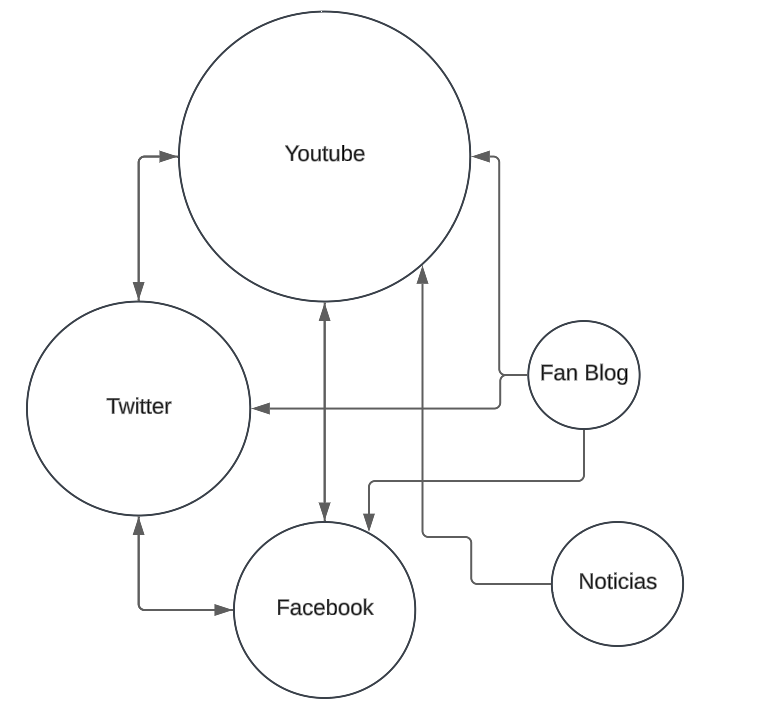
\includegraphics[width=0.7\textwidth]{resources/diagrama1.png}
    \caption{Visualización del grafo dirigido del ecosistema del canal.}
\end{figure}

En el ejemplo, las conexiones fluyen de la siguiente manera:
\begin{itemize}
    \item El canal de YouTube dirige a su Twitter y Facebook. [cite: 15]
    \item El Twitter enlaza hacia el canal de YouTube y el Facebook. [cite: 16]
    \item El Facebook enlaza al Twitter y al canal de YouTube. [cite: 17]
    \item El Fan Blog enlaza al Facebook, al canal de YouTube y al Twitter. [cite: 18]
    \item El post de noticias enlaza únicamente al canal de YouTube. [cite: 19]
\end{itemize}

\subsection{Representación matricial}
Usando este diagrama de conexiones, nos daría la siguiente matriz de adyacencia:
(Recordemos que la primera fila es Youtube, la segunda Twitter, la tercera Facebook, cuarta Fan Blog, quinta Noticias)

\begin{equation}
    A = \begin{pmatrix}
    0 & 1 & 1 & 0 & 0 \\
    1 & 0 & 1 & 0 & 0 \\
    1 & 1 & 0 & 0 & 0 \\
    1 & 1 & 1 & 0 & 0 \\
    1 & 0 & 0 & 0 & 0
    \end{pmatrix} [cite: 20]
\end{equation}

Le aplicamos la lógica de las cadenas de Markov y vemos cómo las fracciones dependen de la cantidad total de hipervínculos de salida en cada página, dándonos esta matriz de transición ($P$):

\begin{equation}
    P = \begin{pmatrix}
    0 & 1/2 & 1/2 & 0 & 0 \\
    1/2 & 0 & 1/2 & 0 & 0 \\
    1/2 & 1/2 & 0 & 0 & 0 \\
    1/3 & 1/3 & 1/3 & 0 & 0 \\
    1 & 0 & 0 & 0 & 0
    \end{pmatrix} [cite: 21]
\end{equation}

\subsection{Iteraciones del algoritmo}
Tomamos nuevamente el ejemplo del diagrama de antes y hacemos las iteraciones. [cite: 22] Para entender de dónde salen los valores de los vectores, realizamos una operación matemática llamada multiplicación de un vector por una matriz. [cite: 23] Para calcular el nuevo puntaje de una página, multiplicamos el vector de probabilidades actual por la columna correspondiente a esa página en la matriz de transición. [cite: 24]

\textbf{1. El punto de partida ($v_0$):}
Iniciamos con un vector donde todos los nodos tienen la misma probabilidad inicial ($1/5$). [cite: 25]
\begin{equation}
    v_0 = \begin{pmatrix} 1/5 & 1/5 & 1/5 & 1/5 & 1/5 \end{pmatrix} [cite: 26]
\end{equation}

\textbf{2. La multiplicación (Producto punto):}
Multiplicamos cada valor de $v_0$ por su valor correspondiente en la primera columna de la matriz $P$ (que contiene las probabilidades de que el resto de las páginas enlacen a YouTube) y sumamos los resultados:
\begin{equation}
    v_1(\text{YouTube}) = \left(\frac{1}{5} \cdot 0\right) + \left(\frac{1}{5} \cdot \frac{1}{2}\right) + \left(\frac{1}{5} \cdot \frac{1}{2}\right) + \left(\frac{1}{5} \cdot \frac{1}{3}\right) + \left(\frac{1}{5} \cdot 1\right) [cite: 27]
\end{equation}

\textbf{3. La suma de fracciones:}
\begin{equation}
    v_1(\text{YouTube}) = 0 + \frac{1}{10} + \frac{1}{10} + \frac{1}{15} + \frac{1}{5}
\end{equation}

Buscando el denominador común (30):
\begin{equation}
    v_1(\text{YouTube}) = 0 + \frac{3}{30} + \frac{3}{30} + \frac{2}{30} + \frac{6}{30} = \frac{14}{30}
\end{equation}

Simplificando la fracción, obtenemos el valor exacto para YouTube en la primera iteración:
\begin{equation}
    v_1(\text{YouTube}) = \frac{7}{15}
\end{equation}

Aplicando este mismo procedimiento para cada columna y repitiéndolo en cada paso, vemos cómo los vectores completos evolucionan en nuestras 3 iteraciones:

\textbf{Iteración 1 ($v_1 = v_0 \cdot P$):}
\begin{equation*}
    v_1 = \begin{pmatrix} \frac{1}{5} & \frac{1}{5} & \frac{1}{5} & \frac{1}{5} & \frac{1}{5} \end{pmatrix} \cdot P = \begin{pmatrix} \frac{7}{15} & \frac{4}{15} & \frac{4}{15} & 0 & 0 \end{pmatrix} [cite: 28]
\end{equation*}

\textbf{Iteración 2 ($v_2 = v_1 \cdot P$):}
\begin{equation*}
    v_2 = \begin{pmatrix} \frac{7}{15} & \frac{4}{15} & \frac{4}{15} & 0 & 0 \end{pmatrix} \cdot P = \begin{pmatrix} \frac{8}{30} & \frac{11}{30} & \frac{11}{30} & 0 & 0 \end{pmatrix}
\end{equation*}

\textbf{Iteración 3 ($v_3 = v_2 \cdot P$):}
\begin{equation*}
    v_3 = \begin{pmatrix} \frac{8}{30} & \frac{11}{30} & \frac{11}{30} & 0 & 0 \end{pmatrix} \cdot P = \begin{pmatrix} \frac{22}{60} & \frac{19}{60} & \frac{19}{60} & 0 & 0 \end{pmatrix}
\end{equation*}

\subsection{Interpretación del ranking obtenido}
Como vemos, el número más grande dentro de los vectores finales es de la página de YouTube ($\frac{22}{60}$). [cite: 29] Esto significa que la página con más relevancia (autoridad) es YouTube, y esto se debe a que es la página que recibe más enlaces importantes hacia ella. [cite: 30] También podemos ver que el Fan Blog y la página de Noticias son equivalentes a 0 en las iteraciones. [cite: 31] Esto se debe a que ninguna de las páginas de la red enlaza hacia ellos, por lo que el "navegante aleatorio" nunca los visita. [cite: 32]